% rara: biber
% arara: xelatex: { synctex: yes }
\documentclass{scrartcl}

\usepackage{amsmath}
\usepackage{amssymb}

\usepackage{tikz}
\usetikzlibrary{calc,shapes,matrix,fit,calc}
\usepackage{pgfplots}
\usepgfplotslibrary{groupplots}
\pgfplotsset{compat=newest}
\usepackage{lscape}


\pgfplotscreateplotcyclelist{algs}{%
	lime!80!black,every mark/.append style={fill=lime},mark=square*\\%
	red,every mark/.append style={fill=red},mark=triangle*\\%
	teal,every mark/.append style={fill=teal!80},mark=pentagon*\\%
	black,mark=star\\%
	purple!30!blue,every mark/.append style={fill=purple!30!blue},mark=diamond*\\%
	orange!80!black,every mark/.append style={solid,fill=orange},mark=*\\%
	yellow!80!black,every mark/.append style={fill=yellow},mark=diamond*\\%
	pink!50!red,every mark/.append style={solid,fill=pink!80!red},mark=*\\%
	purple!80!blue,every mark/.append style={solid,fill=purple},mark=*\\%
}

\pgfplotscreateplotcyclelist{algsbar}{%
	lime!80!black,fill=lime\\%
	red,fill=red\\%
	teal,fill=teal!80\\%
	black,fill=black!80\\%
	purple!30!blue,fill=purple!30!blue\\%
	orange!80!black,fill=orange\\%
	cyan!80!black,fill=cyan\\%
	yellow!80!black,fill=yellow\\%
	pink!80!black,fill=pink\\%
}

\pgfplotsset{
	plotlabels/.style={
			xlabel={Dataset},
			%xlabel style ={yshift=-2cm},
			xtick={
					fib41,
					cere,
					e\_coli,
					influenza,
					para,
					einstein\_de,
					einstein\_en,
					coreutils,
					kernel,
					worldleaders,
				},
			xticklabel style={rotate=-90},%, xshift=0.5cm, yshift=4mm,
		},
	plotticks/.style ={
			symbolic x coords={
					fib41,
					cere,
					e\_coli,
					influenza,
					para,
					einstein\_de,
					einstein\_en,
					coreutils,
					kernel,
					worldleaders,
				},
		}
}

\usepackage{todonotes}
\usepackage{hyperref}
\usepackage{cleveref}

\usepackage{caption}
\usepackage{subcaption}
\usepackage{enumitem}


\newcommand{\lzend}{LZ-End}
\newcommand{\tikzmark}[1]{\tikz[overlay,remember picture] \node (#1) {};}

\usepackage{biblatex}
\addbibresource{Random Access.bib}




\title{Evaluation of Random Access Data Structures for Repetetive Data}
\author{Etienne Palanga}

\begin{document}
\maketitle

\begin{abstract}
	We evaluate several compressed string representations and compare their space consumption in RAM,
	as well as the time required to extract single characters, or substrings of different sizes.
	We also introduce a simple random access data structure based on straight-line grammars.
\end{abstract}

\section{Introduction}

As data volume increasing in almost any field and as such, handling data in compressed form is gaining importance.
The question arises whether text, especially repetetive ones, can be represented in a way which reduces their memory footprint, while still allowing efficient retrieval of the original data.

Approaches to this problem are already known in the literature \cite{belazzougui_block_2021,bille_random_2013,kreft_self-index_2011,nunes_grammar_2022}.
In this short evaluation, we will compare implementations of several compressed data structures.
In this evaluation one is based on context-free grammars, one by \citeauthor{kreft_self-index_2011} is based on the \lzend{} parsing \cite{kreft_self-index_2011}, and another by \citeauthor{belazzougui_block_2021} is based on block trees \cite{belazzougui_block_2021}.

We will evaluate the space requirements as well as query speed for each of the data structures on several repetetive datasets from the Pizza \& Chili Corpus \footnote{\url{http://pizzachili.dcc.uchile.cl/}}.

\section{Data Structures}

For a text $T[1..n] \in \Sigma^n$ with length $n \in \mathbb{N}$ over an alphabet $\Sigma$, we aim to store $T$ in as little space as possible while retaining the ability to access single characters or substrings from $T$.
Various data structures exist to facilitate this.

\subsection{\lzend{}}

One data structure is \citeauthor{kreft_self-index_2011}'s \lzend{}-based data structure.
\lzend{} is a variation of the LZ77 parsing \cite{ziv_universal_1977} in which $T$ is split into phrases $T_f = f_1 f_2 \dots f_k$.
Each phrase $f_i$ is either a single character $c \in \Sigma$ or a pointer to the left in $T$ from which a previously occurring substring is copied. The additional restriction for \lzend{} is that the copied substring must be a suffix of $f_1 \dots f_j$ where $j < i$.
The single character following this copied substring is also part of $f_i$.
An example parsing is given in \cref{fig:02:lzend}, but formal definitions and the specific description of the data structure should be taken from the original paper \cite{kreft_self-index_2011}.
For this evaluation, the parsing is created by \citeauthor{kempa_lz-end_2017}'s implementation \cite{kempa_lz-end_2017}\footnote{\url{https://github.com/dominikkempa/lz-end-toolkit}}.
The random access data structure is generated from this parsing.

\subsection{Block Tree}

The next data structure is the block tree introduced by \citeauthor{belazzougui_block_2021} \cite{belazzougui_block_2021}.
As the name implies, it is a tree-like data structure.
For some parameters $s, \tau \geq 2$, we divide $T$ into $s$ blocks of equal size, then recursively divide the blocks into $\tau$ blocks of equal size.
This procedure is recursively applied to each block, yielding a $\tau$-ary tree, except for the root which has degree $s$.
This tree compressed by identifying blocks, whose content appears to the left of this block on the same level.
Such blocks are replaced by blocks pointing at the previous occurrence.
An example is given in \todo{make block tree figure}.
Again, for formal definitions and explanations of the data structure, we refer to the original paper by \citeauthor{belazzougui_block_2021} \cite{belazzougui_block_2021}.
In this evaluation, an implementation by Reyes\footnote{\url{https://github.com/elarielcl/MinimalistBlockTrees}} is used, which we augmented with support for faster substring operations.\footnote{\url{https://github.com/Skadic/MinimalistBlockTrees}}

\begin{figure}
	\centering
	\begin{equation}
		T_f = b|\tikzmark{anS}a|n|\tikzmark{an}\textcolor{red}{an}a|c|\tikzmark{ana}\textcolor{red}{ana}d|a
	\end{equation}

	\begin{tikzpicture}[overlay, remember picture]
		\begin{scope}[transform canvas={xshift=0.75mm}]
			\draw[->,shorten >=5pt,shorten <=5pt,out=-90,in=-90,distance=0.5cm] (an.north) to (anS.north);
		\end{scope}
		\begin{scope}[transform canvas={xshift=1.25mm}]
			\draw[->,shorten >=5pt,shorten <=5pt,out=-90,in=-90,distance=0.5cm] (ana.north) to (an.north);
		\end{scope}
	\end{tikzpicture}

	\caption{An example of an \lzend{} parsing for $T = bananacanada$. The parts copied from other parts of $T$ are marked in red and their sources are denoted by arrows.}
	\label{fig:02:lzend}
\end{figure}

\subsection{Sampled Scan Grammar}

This is a simple data structure based for strings compressed as straight-line grammars, borrowing definitions from \citeauthor{benz_effective_2013}'s paper \cite{benz_effective_2013}.

\paragraph{Straight-Line Grammars} A \emph{context-free grammar} $G = (\mathcal{N}, \Sigma, P, S)$ is comprised of \emph{non-terminals} $\mathcal{N}$,
\emph{terminals} $\Sigma$ with $\mathcal{N} \cap \Sigma = \emptyset$,
\emph{production rules} $P$ where each rule is of the form $(X \rightarrow \alpha) \in P$ with $X \in \mathcal{N}, \alpha \in (\mathcal{N} \cup \Sigma)^*$.
$X$ is called the \emph{left side} of the rule and $\alpha$ the \emph{right side}.
Lastly, there is a designated \emph{start symbol} $S \in \mathcal{N}$

The expansion $\overset{*}{\rightarrow}$ of a string $(\mathcal{N} \cup \Sigma)^*$ results
by iteratively replacing each non-terminal with a corresponding right side of a rule in $P$
until only terminals remain.
Then we call $L(G) = \{ \alpha\ |\ S \overset{*}{\rightarrow} \alpha \}$, which is the set of all expansions of $S$, the \emph{language} of $G$.

A \emph{straight-line grammar} is a special case of a context-free grammar, where $|L(G)| = 1$.
That is, the grammar only produces one single string. In particular, this also means that the expansion of every non-terminal $X \in \mathcal{N}$ is unique and will be denoted by $ex(X)$.

\paragraph{Sampling} The idea of this data structure is to regularly sample positions in the text and locate them in the grammar, then to save those sample positions.
We sample the positions in such a way, that each sampled position guarantees that we can reach the entirety of the surrounding block from that sample.
When a query is made, we jump to a close sampled position and scan through the grammar for the rest of the way.

Let $T[1..n] \in \Sigma^n$ be a string and $G_T = (\mathcal{N}, \Sigma, P, S)$ a straight-line grammar that produces $T$.
The \emph{sampled scan} data structure saves the number of symbols in each production rule's right side.
For some parameter $r \in \mathbb{N}$ and $r < n$ called the \emph{sampling rate}, we divide $T$ into blocks $T = b_1 \dots b_k$ each of size $r$.

For each block $b_k$, we search for the rule $(X \rightarrow \alpha) \in P$ where $|ex(X)|$ is minimal and $ex(X)$ covers $b_k$ entirely.
We then choose the left-most symbol $c \in \mathcal{N} \cup \Sigma$ in $\alpha$ where $ex(c)$ \emph{starts} inside of $b_k$.
Let $p_\alpha$ be the position of $c$ in $\alpha$ and $p_{b_k}$ the start position of $ex(c)$ in $b_k$. We save the location of $c$ by storing the tuple $s_k := (X, i_\alpha, p_{b_k})$

\subparagraph{Example}

An example is depicted in \cref{fig:02:samplingexample}.
A straight-line grammar for $T = ababacaababa$ and a sampling rate of $r=3$.
and a visual representation are given in \cref{subfig:02:grammar,subfig:02:grammarvisual} respectively.
The sampled symbols are marked in purple.

To calculate the sample for $b_4 = T[10..12]$, we choose the rule that covers it entirely and has a minimally small expansion.
In this case, this is the second $A$. Now we choose the first symbol in that $A$ whose expansion starts in the block $T[10..12]$.
This is the second $B$ in the right side of $A$  at index $3$. Its expansion starts at index $11$ in $T$ which corresponds to index $2$ inside of $T[10..12]$.
This results in the sample: $s_4 = (A, 3, 2)$;

In total we end up with these samples: $(A, 1, 1), (S, 2, 3), (S, 3, 1), (A, 3, 2)$.

\begin{figure}
	\centering
	\begin{subfigure}{0.4\textwidth}
		\centering
		\begin{align*}
			S                   & \rightarrow AcaA \\
			\textcolor{cyan}{A} & \rightarrow aBB  \\
			\textcolor{red}{B}  & \rightarrow ba
		\end{align*}
		\caption{A straight-line grammar for $T$.}
		\label{subfig:02:grammar}
	\end{subfigure}
	\hfill
	\begin{subfigure}{0.5\textwidth}
		\centering
		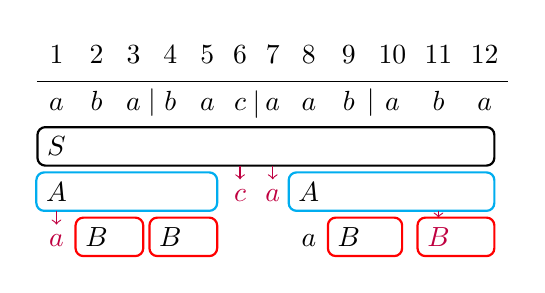
\begin{tikzpicture}
			\node[matrix of nodes, column sep=0mm, row sep=1mm, nodes in empty cells] (m) {
				$1$ & $2$ & $3$ & $4$ & $5$ & $6$ & $7$ & $8$ & $9$ & $10$ & $11$ & $12$\\\hline
				$a$ & $b$ & $a$ & $b$ & $a$ & $c$ & $a$ & $a$ & $b$ & $a$ & $b$ & $a$\\
				$S$ & & & & & & & & & & & \\
				$A$ & & & & & \textcolor{purple}{$c$} & \textcolor{purple}{$a$} & $A$ & & & & \\
				\textcolor{purple}{$a$} & $B$ & & $B$ & & & & $a$ & $B$ & & \textcolor{purple}{$B$} & \\
			};

			% Separators
			\node at ($(m-2-3)!0.5!(m-2-4)$) {$|$};
			\node at ($(m-2-6)!0.5!(m-2-7)$) {$|$};
			\node at ($(m-2-9)!0.5!(m-2-10)$) {$|$};

			\node[fit={(m-3-1.north west) (m-3-12.south east)},
				thick, inner sep=0, rounded corners=1mm,
				draw=black]{};

			\node[fit={(m-4-1.north west) (m-4-5.south east)},
				thick, inner sep=0, rounded corners=1mm,
				draw=cyan]{};
			\node[fit={(m-4-8.north west) (m-4-12.south east)},
				thick, inner sep=0, rounded corners=1mm,
				draw=cyan]{};

			\node[fit={(m-5-2.north west) (m-5-3.south east)},
				thick, inner sep=0, rounded corners=1mm,
				draw=red]{};
			\node[fit={(m-5-4.north west) (m-5-5.south east)},
				thick, inner sep=0, rounded corners=1mm,
				draw=red]{};
			\node[fit={(m-5-9.north west) (m-5-10.south east)},
				thick, inner sep=0, rounded corners=1mm,
				draw=red]{};
			\node[fit={(m-5-11.north west) (m-5-12.south east)},
				thick, inner sep=0, rounded corners=1mm,
				draw=red]{};

			\draw[->,purple] (m-4-1) -- (m-5-1);
			\draw[->,purple] (m-3-6) -- (m-4-6);
			\draw[->,purple] (m-3-7) -- (m-4-7);
			\draw[->,purple] (m-4-11) -- (m-5-11);
		\end{tikzpicture}
		\caption{Visual representation of the grammar.}
		\label{subfig:02:grammarvisual}
	\end{subfigure}
	\caption{An example of sampling with a grammar for the string $T = ababacaababa$. The chosen sampling rate is $r=3$.}
	\label{fig:02:samplingexample}
\end{figure}

\subsubsection{Queries}

Random access and substring queries follow the same general principle.
We choose the sample that lies in the same block as the query index.
From there, we scan until we have found the character or extracted all characters of the substring.

\paragraph{Random Access}

To answer a random access query for $1 \leq i \leq n$, we first determine the block $i$ is contained in, that being $k := \lceil i/r \rceil$.
Let $s_k =: (X, p_{\alpha}, p_{b_k}) \in (\mathcal{N} \cup \Sigma) \times \mathbb{N} \times \mathbb{N}$, where $\alpha$ is the right side of $X$.
Then we know that $\alpha$ contains the character we are looking for since it spans the entire block $b_k$.
Depending on whether $i$ is lesser or greater than $k \cdot r + p_{b_k}$, we now just need to scan either backwards or forwards respectively,
descending into other nonterminals if necessary, in order to find the desired character.
While scanning we skip nonterminals that do not contain $i$ by making use of the saved length of the nonterminals' right side.

\paragraph{Substring}

Answering a substring query for $T[i..j]$ is similar to the random access query.
However, we answer a substring query block-wise. For each block that $T[i..j]$ spans we have a separate query.

For each of these queries we again find the correct sample $s_k$.
We then scan for the positions $i$ and $j$ and while doing so, instead of skipping non-terminals that do not contain $i$ and $j$
we return each terminal we encounter that is in $T[i..j]$.
This of course might require a forward \emph{and} backwards scan each block.

\section{Evaluation}

\todo{add evaluation results and describe them}

In this evaluation we will be comparing the aforementioned data structures and compare their performance and space usage with \texttt{std::string} from the C++ standard library.
The substring queries for \texttt{std::string} do not use the \texttt{substr} method.
Rather, we use the \texttt{std::copy} function to copy the characters into a preallocated \texttt{char} buffer.
Similarly, the queries on the other data structures also copy characters into a preallocated buffer.

The experiments were conducted on a machine running Ubuntu 18.04 with two AMD EPYC 7452 Processors with 32 physical cores (64 logical cores) each running at 2.35GHz base clock rate.

\subsection{Datasets}

All datasets used in this evaluation stem from the Pizza \& Chili repetetive Corpus \footnote{\url{http://pizzachili.dcc.uchile.cl/}}.
Among them are  artificial and real texts.

\paragraph{Artificial}

These are texts that are calculated from a mathematical definition and do not stem from a real-life source.

\begin{itemize}[leftmargin=2cm]
	\item[\textbf{fib41}] If $S_0 = 0$ and $S_1 = 01$ then $S_n = S_{n-1}S_{n-2}$,
		then the concatenation of the previous two words, is called the $n$-th \emph{Fibonacci word}. \cite{barabash_periodic_2016}
		This is $S_{41}$.
\end{itemize}

\paragraph{Real}

These are texts that come from real-live sources and are \emph{not} artificially made repetetive.

\begin{itemize}[leftmargin=2cm]
	\item[\textbf{cere}] $37$ sequences of the yeast \emph{Saccharomyces Cerevisiae}'s genome.
	\item[\textbf{e\_coli}] $23$ sequences of the bacterium \emph{Escherichia Coli}'s genome.
	\item[\textbf{influenza}] $78,041$ sequences of the bacterium \emph{Haemophilus Influenzae}'s genome.
	\item[\textbf{para}] $32$ sequences of the yeast \emph{Saccharomyces Paradoxus}'s genome.
	\item[\textbf{einstein}] All versions of the Albert Einstein Wikipedia article in English and German respectively.
	\item[\textbf{coreutils}] The source code of all 5.x versions of the GNU Coreutils package totalling in 9 versions.
	\item[\textbf{kernel}] The source code of all 1.0.x and 1.1.x versions of the Linux kernel totalling in 36 versions.
	\item[\textbf{worldleaders}] The pdf files of CIA World Leaders from January 2003 to December 2009, converted to text.
\end{itemize}

Statistics concerning each dataset can be found in \cref{tab:03:datastats}.

\begin{table}
	\caption{Statistics for all used datasets.}
	\label{tab:03:datastats}
	\centering
	\begin{tabular}[c]{r|c|c}
		\textbf{Dataset}      & \textbf{Size (MiB)} & \textbf{Alphabet Size} \\\hline\hline
		\textbf{cere}         & $440$               & 5                      \\
		\textbf{e\_coli}      & $108$               & 15                     \\
		\textbf{influenza}    & $148$               & 15                     \\
		\textbf{para}         & $410$               & 5                      \\
		\textbf{einstein\_de} & $89$                & 117                    \\
		\textbf{einstein\_en} & $446$               & 139                    \\
		\textbf{coreutils}    & $196$               & 236                    \\
		\textbf{kernel}       & $247$               & 160                    \\
		\textbf{worldleaders} & $45$                & 89                     \\
	\end{tabular}
\end{table}

% IMPORT-DATA data benches.txt

\subsection{Query Speed}

Random Access (1 character) and substring queries were evaluated.
Each query was run $10^6$ times, and substring queries of lengths $10$, $100$, $1,000$ and $10,000$ were performed.

\subsubsection{Random Access}


Out of the compressed formats, the block tree is the clear winner,
most of the time ahead by several orders of magnitude in comparison to the others.
The results presented for the block tree in \cref{fig:03:raspeed} represent the average for all blocktrees of every used parameterization.

More specific results, can be found in \todo{block tree figure (waiting for random access data for bt zzz...)}

\begin{figure}
	\begin{tikzpicture}
		\begin{axis}[
				title={Random Access},
				width=15cm,
				height=8cm,
				ylabel={Time for $10^{6}$ queries [$\lg_{2}$ ms]},
				legend pos=north east,
				plotticks,
        plotlabels,
				ybar,
				bar width=2mm,
				cycle list name=algsbar
			]
			%% MULTIPLOT(ds) SELECT input_file AS x, AVG(LOG(2, query_time_total)) AS y, MULTIPLOT
			%% FROM data WHERE type='random_access' AND NOT input_file LIKE "%200" GROUP BY filetype, input_file, MULTIPLOT ORDER BY MULTIPLOT,x
			\addplot coordinates { (cere,10.774) (cere,10.733) (coreutils,10.7814) (coreutils,10.5255) (e\_coli,10.668) (e\_coli,9.89482) (einstein\_de,8.88264) (einstein\_de,8.60733) (einstein\_en,8.93958) (einstein\_en,8.99435) (fib41,7.47573) (fib41,7.47573) (influenza,9.90539) (influenza,10.5333) (kernel,10.8865) (kernel,10.6519) (para,10.8634) (para,10.6537) (worldleaders,8.96867) (worldleaders,9.3837) };
			\addlegendentry{ds=sampled\_scan\_512};
			\addplot coordinates { (cere,5.32193) (coreutils,5.2854) (e\_coli,5.20945) (einstein\_de,5.20945) (einstein\_en,5.32193) (fib41,5.24793) (influenza,5.2854) (kernel,5.32193) (para,5.32193) (worldleaders,5.08746) };
			\addlegendentry{ds=string};
		\end{axis}
	\end{tikzpicture}
	\caption{Random access query speed for $10^6$ queries.}
	\label{fig:03:raspeed}
\end{figure}

\subsubsection{Substring}

As depicted in \cref{fig:03:ssspeed}, with substring queries the results are not as conclusive, at least not when looking at the average performance.
In most cases the block tree still beats the grammar.
On very short substrings the block tree is much faster than the grammar in most cases.
The exception here is \textbf{fib41} at which the grammar pulls ahead marginally.

On substrings of length $10,000$ this advantage shrinks significantly.
While the block tree is on average around a factor of $2$ faster than the grammar,
it is still much slower than \texttt{std::string}.
This is usually by a factor of around $2^7$ while the grammar hovers around being around $2^8$
times slower than \texttt{std::string}.
Again, for block trees this plot contains the average across all parameterizations except for the ones saving no extra data to enable faster substring queries.

\begin{figure}
	\begin{tikzpicture}
		\begin{groupplot}[height=25cm,group style={group size= 1 by 2}]
			\nextgroupplot[
				title={Substrings of length $10$},
				width=15cm,
				height=8cm,
				ylabel={Time for $10^{6}$ queries [$\lg_{2}$ ms]},
				legend pos=north east,
				plotticks,
				xtick=\empty,
				ybar,
				bar width=2mm,
				cycle list name=algsbar
			]
			%% MULTIPLOT(ds) SELECT input_file AS x, AVG(LOG(2, query_time_total)) AS y, MULTIPLOT
			%% FROM data WHERE type='substring' AND NOT input_file LIKE "%200" AND substring_length=10 AND ((prefix_suffix is null) or (not prefix_suffix=0)) GROUP BY filetype, input_file, MULTIPLOT ORDER BY MULTIPLOT,x
			\addplot coordinates { (cere,8.43755) (coreutils,8.56445) (e\_coli,8.25194) (einstein\_de,8.20461) (einstein\_en,8.36463) (fib41,8.59862) (influenza,8.03316) (kernel,8.48142) (para,8.38883) (worldleaders,8.08476) };
			\addlegendentry{ds=blocktree};
			\addplot coordinates { (cere,11.0841) (cere,11.1046) (coreutils,11.1799) (coreutils,11.1222) (e\_coli,11.0133) (e\_coli,10.4988) (einstein\_de,9.5411) (einstein\_de,9.41574) (einstein\_en,9.66) (einstein\_en,9.70908) (fib41,8.33539) (fib41,8.37938) (influenza,10.3151) (influenza,11.0007) (kernel,11.2432) (kernel,11.1755) (para,11.1674) (para,11.032) (worldleaders,9.59991) (worldleaders,10.021) };
			\addlegendentry{ds=sampled\_scan\_512};
			\addplot coordinates { (cere,5.75489) (coreutils,5.72792) (e\_coli,5.64386) (einstein\_de,5.64386) (einstein\_en,5.75489) (fib41,5.70044) (influenza,5.70044) (kernel,5.72792) (para,5.72792) (worldleaders,5.52356) };
			\addlegendentry{ds=string};

			\nextgroupplot[
				title={Substrings of length $10,000$},
				width=15cm,
				height=8cm,
				ylabel={Time for $10^{6}$ queries [$\lg_{2}$ ms]},
				legend pos=north east,
				plotticks,
				plotlabels,
				ybar,
				bar width=2mm,
				cycle list name=algsbar
			]
			%% MULTIPLOT(ds) SELECT input_file AS x, AVG(LOG(2, query_time_total)) AS y, MULTIPLOT
			%% FROM data WHERE type='substring' AND NOT input_file LIKE "%200" AND substring_length=10000 AND ((prefix_suffix is null) or (not prefix_suffix=0)) GROUP BY filetype, input_file, MULTIPLOT ORDER BY MULTIPLOT,x
			\addplot coordinates { (cere,17.2475) (coreutils,17.3947) (e\_coli,17.137) (einstein\_de,17.399) (einstein\_en,17.4904) (fib41,17.8324) (influenza,16.8642) (kernel,17.4573) (para,17.1411) (worldleaders,17.2921) };
			\addplot coordinates { (cere,18.2669) (cere,18.419) (coreutils,18.307) (coreutils,18.7239) (e\_coli,18.3196) (e\_coli,18.3401) (einstein\_de,17.8303) (einstein\_de,17.793) (einstein\_en,17.8559) (einstein\_en,17.9275) (fib41,16.836) (fib41,16.8349) (influenza,17.8795) (influenza,18.5641) (kernel,18.2382) (kernel,18.628) (para,18.4188) (para,18.3881) (worldleaders,17.5317) (worldleaders,17.7543) };
			\addplot coordinates { (cere,9.93369) (coreutils,9.83763) (e\_coli,9.75322) (einstein\_de,9.72622) (einstein\_en,9.90689) (fib41,9.87191) (influenza,9.80574) (kernel,9.86264) (para,9.93221) (worldleaders,9.49386) };

		\end{groupplot}
	\end{tikzpicture}
	\caption{Substring query speed for $10^6$ queries.}
	\label{fig:03:ssspeed}
\end{figure}

In \cref{fig:03:ssspeedbt} results for the different parameterizations of block trees are depicted.
The arity (A in the figure) refers to the number of nodes that each block is recursively divided in.
The prefix/suffix size (PS in the figure) is the number $k$ such that each block in the tree saves its first and last $k$ characters each, to facilitate faster substring queries.
For the exact workings of the query, we refer to the original paper by \citeauthor{belazzougui_block_2021} \cite{belazzougui_block_2021}.

\begin{figure}
	\begin{tikzpicture}
		\begin{groupplot}[height=25cm,group style={group size= 1 by 2}]
			\nextgroupplot[
				title={Substrings of length $10$},
				width=15cm,
				height=8cm,
				ylabel={Time for $10^{6}$ queries [$\lg_{2}$ ms]},
				legend pos=north east,
				plotticks,
				xtick=\empty,
				ybar,
				bar width=1.5mm,
				cycle list name=algsbar
			]
			%% MULTIPLOT(ds,arity,prefix_suffix) SELECT input_file AS x, AVG(LOG(2, query_time_total)) AS y, MULTIPLOT
			%% FROM data WHERE type='substring' AND NOT input_file LIKE "%200" AND substring_length=10 AND (not prefix_suffix=0 or ds='string') GROUP BY filetype, input_file, MULTIPLOT ORDER BY MULTIPLOT,x
			\addplot coordinates { (cere,9.59897) (coreutils,9.82879) (e\_coli,9.52913) (einstein\_de,9.66734) (einstein\_en,9.85104) (fib41,10.024) (influenza,9.2275) (kernel,9.83453) (para,9.59932) (worldleaders,9.55067) };
			\addlegendentry{ds=blocktree,arity=2,prefix\_suffix=4};
			\addplot coordinates { (cere,8.34207) (coreutils,8.48985) (e\_coli,8.22159) (einstein\_de,8.18982) (einstein\_en,8.36412) (fib41,8.47168) (influenza,7.92777) (kernel,8.46556) (para,8.29691) (worldleaders,8.07142) };
			\addlegendentry{ds=blocktree,arity=2,prefix\_suffix=16};
			\addplot coordinates { (cere,8.1541) (coreutils,8.26343) (e\_coli,7.86274) (einstein\_de,7.91317) (einstein\_en,8.04882) (fib41,8.56795) (influenza,7.66521) (kernel,8.17628) (para,8.04939) (worldleaders,7.70784) };
			\addlegendentry{ds=blocktree,arity=32,prefix\_suffix=4};
			\addplot coordinates { (cere,7.65506) (coreutils,7.67575) (e\_coli,7.39431) (einstein\_de,7.04811) (einstein\_en,7.19455) (fib41,7.33089) (influenza,7.31217) (kernel,7.4493) (para,7.6097) (worldleaders,7.0091) };
			\addlegendentry{ds=blocktree,arity=32,prefix\_suffix=16};
			\addplot coordinates { (cere,5.75489) (coreutils,5.72792) (e\_coli,5.64386) (einstein\_de,5.64386) (einstein\_en,5.75489) (fib41,5.70044) (influenza,5.70044) (kernel,5.72792) (para,5.72792) (worldleaders,5.52356) };
			\addlegendentry{ds=string,arity=,prefix\_suffix=};

			\nextgroupplot[
				title={Substrings of length $10,000$},
				width=15cm,
				height=8cm,
				ylabel={Time for $10^{6}$ queries [$\lg_{2}$ ms]},
				legend pos=north east,
				plotticks,
				plotlabels,
				ybar,
				bar width=1.5mm,
				cycle list name=algsbar
			]
			%% MULTIPLOT(ds,arity,prefix_suffix) SELECT input_file AS x, AVG(LOG(2, query_time_total)) AS y, MULTIPLOT
			%% FROM data WHERE type='substring' AND NOT input_file LIKE "%200" AND substring_length=10000 AND (not prefix_suffix=0 or ds='string') GROUP BY filetype, input_file, MULTIPLOT ORDER BY MULTIPLOT,x
			\addplot coordinates { (cere,18.8403) (coreutils,19.1041) (e\_coli,18.8392) (einstein\_de,19.0291) (einstein\_en,19.1602) (fib41,19.4844) (influenza,18.4945) (kernel,19.1322) (para,18.7615) (worldleaders,19.005) };
			\addplot coordinates { (cere,17.1538) (coreutils,17.2951) (e\_coli,17.087) (einstein\_de,17.2565) (einstein\_en,17.3388) (fib41,17.6107) (influenza,16.8231) (kernel,17.3243) (para,17.0559) (worldleaders,17.2475) };
			\addplot coordinates { (cere,17.0671) (coreutils,17.225) (e\_coli,16.8793) (einstein\_de,17.2456) (einstein\_en,17.3977) (fib41,17.8574) (influenza,16.5579) (kernel,17.3413) (para,16.9123) (worldleaders,17.021) };
			\addplot coordinates { (cere,15.9288) (coreutils,15.9545) (e\_coli,15.7424) (einstein\_de,16.0647) (einstein\_en,16.0647) (fib41,16.3773) (influenza,15.5812) (kernel,16.0314) (para,15.8348) (worldleaders,15.8949) };
			\addplot coordinates { (cere,9.93369) (coreutils,9.83763) (e\_coli,9.75322) (einstein\_de,9.72622) (einstein\_en,9.90689) (fib41,9.87191) (influenza,9.80574) (kernel,9.86264) (para,9.93221) (worldleaders,9.49386) };

		\end{groupplot}
	\end{tikzpicture}
	\caption{Substring query speed for $10^6$ queries.}
	\label{fig:03:ssspeedbt}
\end{figure}


\section{Conclusion}

\include{bib.tex}

\end{document}
